\subsection{Das Mathematik-Paket}
\textit{Mathematik-Paket} ist der interne Name für diejenige Software Komponente, die alles in Bezug auf mathematische Vorgänge verarbeitet. Aus dem Versuch, diese Komponente in Programmcode zu fassen, erlangte ich eine wesentliche Erkenntnis: Theoretische Mathematik und Informatik sind viel weiter voneinander entfernt, als man glauben mag.\\\\
In der Mathematik sieht man Konstrukte als abstrakt, soweit sollte die mathematische Sicht der Dinge ja bekannt sein. Durch Definitionen schafft sich ein Mathematiker Freiraum, wodurch auch der Level der Abstraktion steigt. Zum Beispiel ist uns möglicherweise nicht sofort bewusst, dass wir beim 'mit $x$ multiplizieren' tatsächlich $x$-Mal zusammenzählen. Beim 'hoch $x$ rechnen' wird eigentlich $x$-Mal multipliziert, also wie oft addiert? Natürlich stellen die Grundrechenarten programmtechnisch kein Problem dar, jedoch ist bereits diese einfache Frage ohne mehr Information nicht zu beantworten, was zeigen soll, wie tief wir bereits drin stecken, ohne jemals angefangen zu haben.\\\\
In diesem Teil der Programmierung geht es also darum, die abstrakten mathematischen Beschreibungen der Dinge in konkretisierte, ausführbare, Programmstücke zu fassen. Zuerst haben wir uns ein Grundkonzept überlegt, das folgenden Anforderungen entsprechen sollte:
\begin{itemize}
	\item Alle Mathematischen Vorgänge sollen abbildbar sein
	\begin{itemize}
		\item Rechnungen
		\item Gleichungen
		\item Funktionen/Variablendefinitionen
		\item Gleichungssysteme
	\end{itemize}
	\item geringer \textit{RAM}-Aufwand (Arbeitsspeicher)
	\item durch geringen Aufwand änderbar
	\item durch geringen Aufwand durchsuchbar
\end{itemize}
Der Grund für die notwendige Änderungsfähigkeit ist ganz einfach, dass der Benutzer zu jedem Zeitpunkt in der Lage sein soll, die Eingabe zu bearbeiten. Die Suchfunktion ist erklärbar, wenn man einen Schritt weiter denkt: mathematische Funktionen sowie andere Vorgänge müssen unvermeidlich die zu ersetzenden Variablen ausfindig machen und stattdessen Zahlen einfügen. Ich spreche hier "andere Vorgänge" an, da beispielsweise Gleichungssysteme oder das einfache Einsetzen von Variablen diese Funktionalität ebenfalls gebrauchen könnten, das hängt jedoch von der Implementierung ab.\\
Schlussendlich fanden wir zwei Lösungen, die für die engere Auswahl in Frage kamen:\\
\\
Lösung 1: Gesamte Information in einen \textit{String}  verpacken, etwa so, dass $2 \cdot x+3 $ als \textbf{" \textbackslash Sum( \textbackslash Product( \#2, \_x ), \#3)"} gespeichert wird. Ein \textit{String} unterscheidet sich im Wesentlichen nicht von einem Text im Programmier-Jargon (der Ausdruck stammt von "Zeichenkette" ab).\\
\\
Lösung 2: Struktur wird per \textit{Objekt(e)} gespeichert. Jedes Objekt sollte für eine Operation oder etwas Vergleichbares stehen. Hier wäre unser Term $2 \cdot x+3 $, wenn so dargestellt, dass die Eigenschaften eines Objektes darunter aufgelistet sind, Folgendes:\\
\textbf{
\begin{itemize}
	\item[$-$] Sum
	\begin{itemize}
		\item[$-$] Product
		\begin{itemize}
			\item[$-$] Constant: $2.0$
			\item[$-$] Variable: $x$
		\end{itemize}
		\item[$-$] Constant: $3.0$
	\end{itemize}
\end{itemize}
}
\ \\
Variante 1 hatte den wesentlichen Vorteil, dass suchen und ersetzen äußerst einfach gewesen wären, da Java für Strings schon standardmäßig Funktionen hierfür anbietet. Wie man sehen kann, ist die erste Version auch kompakter, dafür kann sie mit Struktur nicht punkten: Wo ein bestimmtes Element beginnt und endet ist nirgends hinterlegt, dies dürfte also bei jedem Durchgang aufs Neue ermittelt werden. Das entscheidende Argument für die Objekt-Struktur war letztendlich, dass die Modularität viel präziser ablaufen könnte. Das kann man sich so vorstellen, dass, um Strings zu verarbeiten sinnvollerweise eine zentrale Stelle (gemeint: \textit{Methode}) für die Interpretation verantwortlich ist. Das bedeutet, dass sich sämtliche Erweiterungen an die Regeln dieser Stelle halten müssten. Bei Variante 2 hingegen wären sämtliche Funktionen ausgelagert, sprich: jedes Objekt arbeitet nach Belangen, solange globale Anforderungen erfüllt werden. Mit "Anforderungen" ist hier einfach gemeint, dass es berechenbar ist, in der Lage ist, Variablen zu ersetzen usw.\\
\subsubsection{Term-Struktur}
Die Wahl fällt also eindeutig auf die oben angeführte Lösung Nr. 2, sie ist flexibler, strukturierter und modularer als ihre Alternative. In der Code-Implementierung bietet es sich an, sich die \textit{Vererbung} zu Nutze zu machen. Das bedeutet in Java, dass eine \textit{Mutterklasse} (auch: \textit{Überklasse}) existiert, die so etwas wie ein Gerüst vorgibt. Ich verwende hier bewusst nicht den Ausdruck "Grundgerüst", da auch Mutterklassen weitere Mutterklassen haben können, wobei jede Ebene zum letzten Objekt der Kette beiträgt. Solch eine Überklasse muss einfach mit dem Schlüsselwort \displaycode{abstract} gekennzeichnet werden und darf praktisch die Umrisse für alle Methoden enthalten, obwohl sie keine einzige genau beschreiben muss. Das hat den Sinn, dass Objekte klassifiziert werden können und trotzdem ihre Funktionalität eigenständig verwalten dürfen.\\
\\
Im konkreten Fall bedeutet dies nun, dass wir eine abstrakte Mutterklasse \displaycode{Term} geschrieben haben, die - sehr unspektakulär - mathematische Terme (Ausdrücke) darstellen soll. Ein Term ist alles von Summe über Bruch, Logarithmus bis zur einfachen Konstante. Hinter der \displaycode{Constant} ($\rightarrow$ Konstante) verbirgt sich nichts anderes als eine Zahl, wir dachten jedoch, der Name würde besser im Kontrast zur \displaycode{Variable} ($\rightarrow$ Variable) stehen. Diese Klasse legt nun einige abstrakte Methoden fest, wie zum Beispiel \displaycode{public Term calc()}, in der das jeweilige Unterobjekt seinen Inhalt berechnen und zurückgeben soll. Die gleiche Methode gibt es auch mit Parameter, nämlich einem Objekt, das alle aktuellen Variablenwerte hält, was eben für Funktionen wichtig wäre. Als kurze Veranschaulichung würde diese Methode zum Beispiel bei der \displaycode{Sum} ($\rightarrow$ Summe) ganz einfach so aussehen, dass sie alle ihre Summanden auffordert, deren Inhalt zu berechnen und diese im Anschluss addiert.\\
\\
Die nächste Anforderung war, dass sie neben einigen Methoden, die ich bis jetzt noch nicht erwähnt habe, wie \displaycode{void simplify()} zum vereinfachen oder \displaycode{void changeSubterm(Term o, Term n)} aus strukturtechnischen Gründen, zusätzlich eine Funktionalität zum Ableiten nach einer Variable besitzen. Ich werde nun die Implementation der Methode \displaycode{Term derive()} in der Klasse \displaycode{Sum} demonstrieren. In der Arbeit wurde dies natürlich für alle Unterklassen fertiggestellt. Hier nun die Ableitungsregel für Summen:
\begin{gather*}
\frac{d(f(x)+g(x)}{dx} = \frac{d f(x)}{dx}+\frac{d g(x)}{dx}
\end{gather*}
Der Java-Code liest sich folgendermaßen:\\

\begin{center}
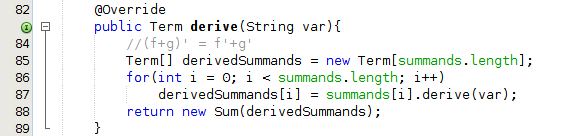
\includegraphics[width=0.9\textwidth]{img/sachsenschnitzel/code_Sum_derive_cropped}
\end{center}
\noindent
Ich denke an diesem Beispiel kann man äußerst klar erkennen, dass die Wahl unserer derzeitigen Struktur zu einigen guten Ergebnissen geführt hat. Der Programmcode ist gekapselt, modular und einfach lesbar.
%klammern? nicht-wirklich-terme?

\subsubsection{Terme, Funktionen, Gleichung(ssysteme)}
Die Terme wären hiermit soweit abgedeckt, was allerdings tun mit Gleichungen? Sind Gleichungen nicht eigentlich auch Terme?\\
Beim weiteren Nachdenken fällt auf, dass Terme der Bedingung gehorchen, dass man sie schachteln kann, so kann eine Summe beispielsweise weitere Summen, genauso aber Konstanten oder jede andere Art von Term beinhalten. Zusammengefasst sind ihre Summanden also einfach weitere Terme, die beliebig tief geschachtelt sein dürfen. Unsere anfängliche Frage sollte nun einfach zu klären sein: kann eine Summe eine Gleichung beinhalten? Nein. Auf diese Antwort hätte man genauso in der Mathematik stoßen können: Laut Definition ist eine Gleichung eine \citebrackets{Aussage über die Gleichheit zweier Terme} und \citebrackets{entweder wahr oder falsch}\footcite{math_gleichung} und ist damit selbst kein Term, da in der Mathematik niemand mit einer wahr/falsch-Information weiter rechnen kann.\\
\\
In diesem Sinne wurden Gleichungen logischerweise implementiert, sie besitzen zwei Terme, über die sie verfügen können. Aber was nun ist mit Funktionen? Funktionen scheinen berechenbar. Allerdings sollte man hier vorsichtig sein, denn streng genommen kann man, ähnlich wie in der Informatik, zwischen zweierlei Verwendung der Funktionen unterscheiden: Auf der einen Seite spricht man von der Definition der Funktion, der Teil, bei dem man etwa $f(x) = 2 \cdot x  - 4$ schreibt, um anzuzeigen, was in der Funktion passieren soll. Aber wann soll das passieren? Damit wären wir bei der anderen Anwendung, wo eine Funktion verwendet oder \textit{aufgerufen} wird. Hier könnte zum Beispiel $f(x=3)$ das Ergebnis $2 \cdot 3 - 4 = 2$ liefern. Im Endeffekt werden im Programmcode also beide Varianten benötigt, von welchen eine ein \displaycode{Term} und die andere kein solcher sein soll. Die Funktionsdefinition sieht sogar eher einer Gleichung ähnlich, im Endeffekt wird sie immerhin dargestellt als $<Funktionsname>(<Funktionsvariable(n)>)=<Funktionsterm>$.\\
\\
Da Gleichungen ja bereits behandelt wurden, ist es ziemlich offensichtlich, dass Gleichungssysteme ebenfalls keine Untergruppe der Terme darstellen. Sie werden ganz einfach mehrere Gleichungen beinhalten und eine Funktionalität zum Auslesen der \textit{Koeffizienten} (=Zahlen vor einzelnen Variablen) besitzen, was später noch von Bedeutung sein wird.\\
\\
Unserer Meinung nach ist es sinnvoll, auch für diese mathematischen Objekte einen gemeinsamen Nenner zu finden. Warum wir so entschieden haben, wird sich in weiteren Kapiteln noch zeigen. Also haben wir kurzerhand die Klasse \displaycode{MathObject} ins Leben gerufen. Sie soll, wie der Name bereits verrät, als Über-Objekt für alle mathematischen Konstrukte wirken, sodass \displaycode{Term}, \displaycode{Function}, \displaycode{Equation} und \displaycode{SystemOfEquations} \textit{Child-Objekt} davon sind.

\section{Lösung linearer Gleichungssysteme in Java}
Da nun Objektstruktur und Vererbung geklärt sind, besteht der nächste Schritt darin, Berechnungen durchzuführen. Als Einstieg in das Thema möchte ich mit Gleichungssystemen beginnen. \textit{Lineare Gleichungssysteme} zu lösen haben die meisten sicher in der Schule gelernt. Das sind zur Erinnerung jene, bei denen lediglich konstante Koeffizienten vor den Variablen stehen, womit Ausdrücke wie $ln(x)$ oder $x^2$ ausgeschlossen sind. Damit das hier ein wenig anschaulicher wird, werde ich für das gesamte Kapitel folgendes Beispiel-Gleichungssystem verwenden:\\
\begin{gather*}
2x + 4y - z = 17\\
x + 3y + 2z = 18\\
-7x + 5y + z = -29
\end{gather*}
\noindent
Nun gibt es verschiedene Möglichkeiten, Gleichungssysteme zu lösen. Einsetz- oder Substitutionsverfahren, Additionsverfahren, Matrixverfahren sind vielleicht gängige Namen, über die man in diesem Bereich stolpern könnte. Am besten eignet sich für den Computer natürlich eines, bei dem möglichst viel mit Zahlen allein gemacht werden kann. Da das Substitutionsverfahren darauf beruht, dass einzelne Variablen durch andere dargestellt werden können, bis bloß eine übrig ist, scheidet dieses aus. Beim Matrixverfahren wird die Inverse von Matrizen benötigt, deren Berechnung wir als aufwendiger erachteten als das gaußsche Eliminationsverfahren, in dem einfach eine Gleichung nach der anderen gekürzt wird, bis alles von unten aufgelöst werden kann. Dieses Verfahren werde ich nun demonstrieren und anschließend den Programmcode zeigen.\\
Deutlich aufgelistet sieht unser Gleichungssystem folgendermaßen aus:

\[ %Ausgangssystem
\systeme{
	2x  +  4y  -   z  =  17,
	 x  +  3y  +  2z  =  18,
	-7x +  5y  +   z  = -29}
\]

\[ %auf gleich multiplizieren #1
\systeme{
	2x  +  4y  -   z  =  17,
	2x  +  6y  +  4z  =  36,
	2x - \frac{10}{7}y - \frac{2}{7}z = \frac{58}{7}}
\]

\[ %subtraktion #1
\systeme{
	2x  +  4y  -   z  =  17,
	       2y  +  5z  =  19,
		   \frac{38}{7}y  -  \frac{5}{7}z  = \frac{61}{7}}
\]

\[ %auf gleich multiplizieren #2
\systeme{
	2x  +  4y  -   z  =  17,
		   2y  +  5z  =  19,
		   2y  -  \frac{5}{19}z  = \frac{61}{19}}
\]

\[ %subtraktion #2
\systeme{
	2x  +  4y  -   z  =  17,
		2y  +  5z  =  19,
			\frac{100}{19}z  = \frac{300}{19}}
\]

%TODO: von unten nach oben auflösen

Das Verfahren findet man zudem äußerst gut dokumentiert auf der Webseite von Dieter Heidorn\footcite{math_gauss_verfahren}. %Webseite drin lassen???